\documentclass[10pt,twocolumn]{article}
\usepackage[margin=0.5in]{geometry}
\usepackage[cmex10]{amsmath}
\usepackage{amsmath}
\usepackage{amsmath,amssymb,amsfonts}
\usepackage{graphicx}
\usepackage{textcomp}
\usepackage{amsmath,amssymb,amsfonts,amsthm}
\usepackage{gensymb}
\usepackage{mathtools}
\newcommand*{\Comb}[2]{{}^{#1}C_{#2}}%
\title{
Probability Assignment
}
\author{GINNA SHREYANI}
\date{}
\begin{document}
\maketitle


\textbf{11.16.3.2}\\
A coin is tossed twice, what is the probability that atleast one tail occurs?\\
\subsection*{Solution}
By using binomial distribution we can find the probability of atleast one tail occurs hen a coin is tossed twice.\\
The Binomial Distribution: Let
\begin{align}
	&Y = \sum_{i=1}^n X_i
     \label{eq-1}
\end{align}
where n is the total number of times the coin is tossed. Then X has a binomial distribution. Then, for
\begin{align}
	&p_{X_i}(n){\stackrel{z}{\rightleftharpoons}}P_{X_i}(z),
     \label{eq-2}
\end{align}
yielding
\begin{align}
	&P_{X_i}(Z)= 1-p+pz^{-1}
	\label{eq-3}
\end{align}
Since $X_i$ are i.i.d.,
\begin{align}
	P_X(Z)&=(1-p+pz^{-1})^n\\
	&=\sum_{k=0}^n{\Comb{n}{k}p^{k}(1-p)^{n-k}}
\end{align}
\[
	p_X(k)=
	\begin{cases}
		\Comb{n}{k}p^{n-k}(1-p)^k,& \text{if } 0\leq k\leq n\\
		0,& \text{otherwise}
	\end{cases}
\]
As a result it is written as
\begin{align}
	\label{eq-6}
	&p_X(k)=\binom nk p^{k}(1-p)^{n-k}
\end{align}
The cumulative distribution function of X is defined as
\begin{align}
	&F_X(r)=P_r(X\leq r) = \sum_{k=0}^r\binom nk p^{k}(1-p)^{n-k}
	\label{eq-7}
\end{align}
Therefore, we get the number of trails i.e., the number of times the coin is tossed and the probability of getting atleast one tail is sum of the probability of getting one tail and probability of getting two tails.
The probability of getting a tail when a coin is tossed is 0.5.
\begin{align*}
	&n = 2\\
	&r = 1,2\\
	&p = 0.5\\
\end{align*}
Therefore,
\begin{align}
	P(Y\geq 1)&=\sum_{k=1}^2 \binom nk p^k(1-p)^{n-k}\\
	&=\binom 21(0.5)^1(1-0.5)^{2-1}+\binom 22 (0.5)^2(1-0.5)^{2-2}\\
	P(Y\geq 1)&=0.5+0.25\\
	P(Y\geq 1)&= 0.75
\end{align}
Therefore,the probability of getting atleast one tail whenthe coinis tossed twice is 0.75.\\ 
\begin{figure}[h]
    \centering
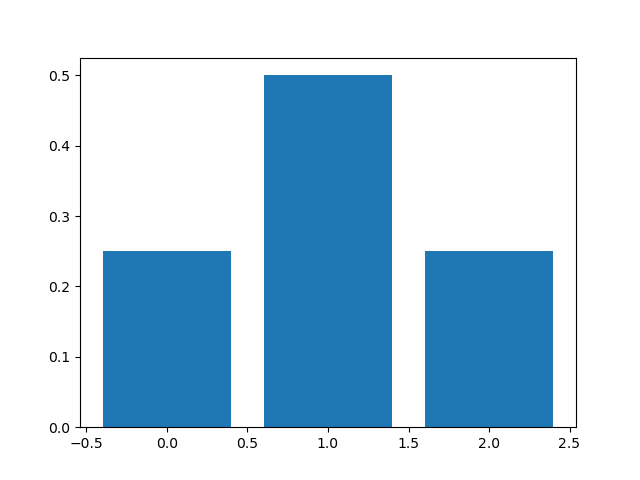
\includegraphics[width=\columnwidth]{fig/11.16.3.2.png}
\end{figure}\\


This is the code\\
\href{https://github.com/ShreyaniReddy/IITH-FWC/blob/main/probability/11.16.3.2/codes/11.16.3.2.py}


\end{document}
